\subsubsection{Bild-basierte Rechnungsklassifizierung}
\label{chap:image-recon}
% http://citeseerx.ist.psu.edu/viewdoc/download?doi=10.1.1.414.9846&rep=rep1&type=pdf

% Analog der Klassifizierung von Objekten auf Fotos, ist es auch denkbar, Rechnung mit Hilfe diesem Bild-basiertem Vorgehen zu klassifizieren.

Dieses Kapitel erläutert ein Experiment, bei welchem Algorithmen und Modelle aus dem Bereich der Computer Vision angewendet werden, um Rechnungen zu klassifizieren.

% ResNet Arxiv: https://arxiv.org/abs/1512.03385
% ResNet: https://towardsdatascience.com/an-overview-of-resnet-and-its-variants-5281e2f56035
% DRM Arxiv: https://arxiv.org/abs/1512.03385
% DRN: https://towardsdatascience.com/review-drn-dilated-residual-networks-image-classification-semantic-segmentation-d527e1a8fb5
% InceptionV4: https://towardsdatascience.com/review-inception-v4-evolved-from-googlenet-merged-with-resnet-idea-image-classification-5e8c339d18bc

% NASNet: https://ai.googleblog.com/2017/11/automl-for-large-scale-image.html

% NASNet example https://www.tensorflow.org/hub/tutorials/image_retraining

% AutoML: https://ai.googleblog.com/2017/05/using-machine-learning-to-explore.html


% TODO: Dilated Residual Network beschreiben: Veränderung der Convolutions in einem ResNet zu einem Grid anstelle der herkömmlichen convolution.

Im Folgenden wird das ResNet, das Inception-ResNet-V2 sowie das NASNet large Netzwerk angewendet, um die bisher bei der AXA eingereichten Rechnung zu klassifizieren.

Um Objekterkennungsmodelle mit Millionen von Parametern zu trainieren, werden viele Trainingsdaten und eine enorme Kapazität an Rechenleistung benötigt. Das Konzept des Transfer Learning bietet die Möglichkeit, diese beiden Problematiken zu Umgehen und dabei nur wenige oder keine Einbussen bei der Trefferquote verzeichnen zu müssen (vgl. Kapitel \ref{chap:transfer-learning}). % \autocite{TensorflowImageRetraining}

Um die Rechnungen zu klassifizieren wird Transfer Learning angewendet, indem die genannten Modelle auf dem ImageNet Datensatz trainiert werden, bevor die eigentliche Problemstellung angegangen wird.

Nach dem Training auf dem ImageNet Datensatz werden die letzten Schichten des Netzwerks, jene die für die Klassifizierung zuständig sind, durch ein neues Klassifizierungsnetzwerk ersetzt. Dadurch wird der Trainingseffekt durch den ImageNet Datensatz beibehalten und die Klassifizierung so angepasst, dass sie die Einteilung in die vier vorliegenden Klassen erlaubt.

Die Abbildung \ref{image-classification-model} zeigt die Klassifizierungsmodelle, welche zur Anwendung kommen. Input ist jeweils der Feature-Vektor, welcher durch das ResNet, Inception-ResNet beziehungsweise NASNet Netzwerk erstellt wurde. Beim ResNet und Inception-ResNet wird dieser Feature-Vektor durch ein Convolution und ein Flatten Layer in einen eindimensionalen Vektor gebracht. Das NASNet liefert bereits einen eindimensionalen Feature-Vektor und die ersten zwei Schichten entfallen. Durch zwei Hidden Layer wird der Vektor schlussendlich zu einem One-Hot Encoded Vektor für die vier Klassen reduziert. Zwischen den Hidden Layern sind zwei Dropout Layer zur Reduzierung des Overfitting eingeschoben.


\begin{figure}[h!] 
  \captionsetup{width=.9\linewidth}
  \caption{neuronale Netze, welche bei der Bild-basierten Klassifizierung zur Anwendung kommen}
  \label{image-classification-model} 
  \begin{subfigure}[b]{0.3\linewidth}
    \centering
    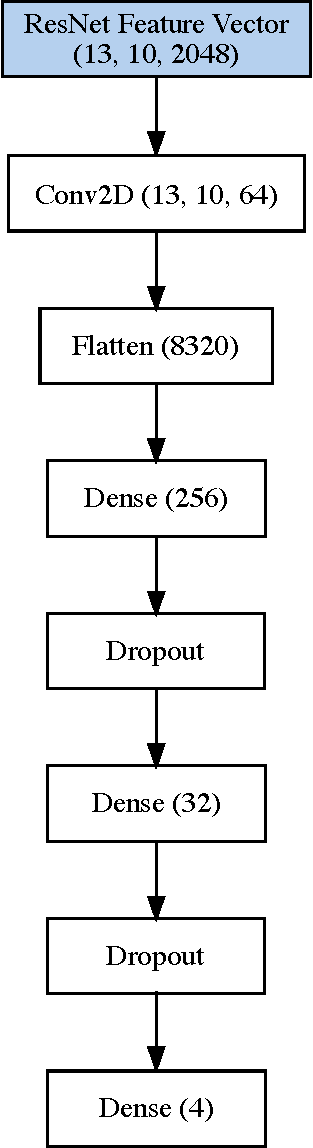
\includegraphics[scale=0.6]{graphics/image-classification-results/model/resnet.pdf} 
    \caption{ResNet} 
    \label{image-classification-model:resnet} 
    \vspace{2ex}
  \end{subfigure}%% 
   \begin{subfigure}[b]{0.3\linewidth}
    \centering
    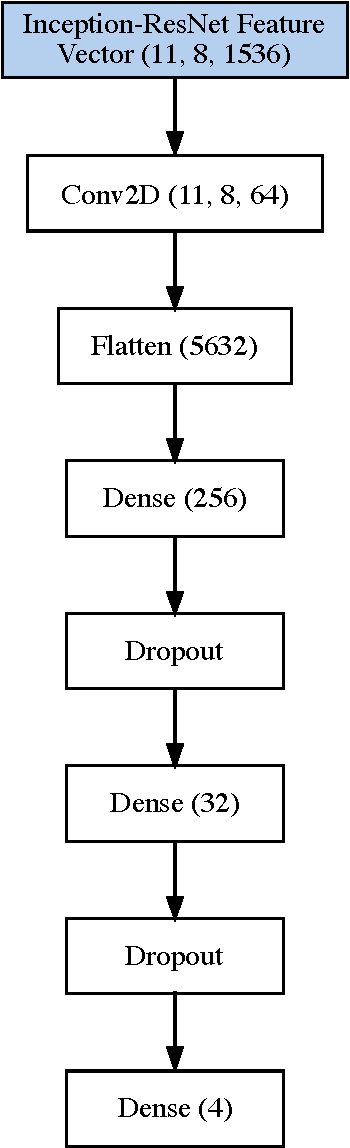
\includegraphics[scale=0.6]{graphics/image-classification-results/model/inception.pdf} 
    \caption{Inception-ResNet-V2} 
    \label{image-classification-model:inception} 
    \vspace{2ex}
  \end{subfigure}%% 
  \begin{subfigure}[b]{0.3\linewidth}
    \centering
    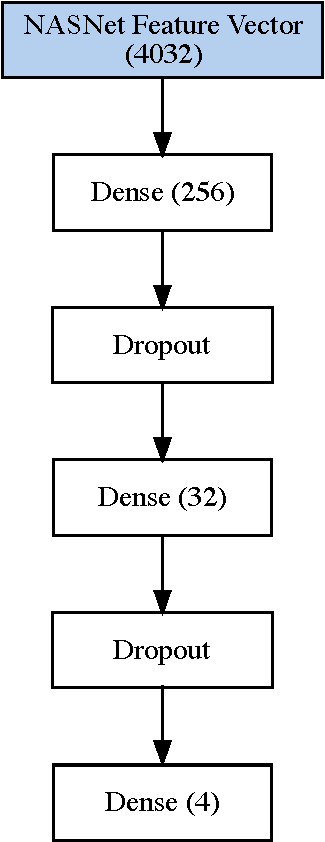
\includegraphics[scale=0.6]{graphics/image-classification-results/model/nasnet.pdf} 
    \caption{NASNet} 
    \label{image-classification-model:nasnet} 
    \vspace{2ex}
  \end{subfigure} 
  \centering
\end{figure}

Die genannten Modelle werden mit 80\% der vorhandenen Daten trainiert, die übrigen 20\% werden benötigt, um den Trainingsfortschritt zu prüfen. Mit diesen 20\% Testdaten soll ein allfälliges Overfitting erkannt werden.

Die Abbildung \ref{image-class-results} zeigt das Training der genannten Modelle während 60 Trainingsepochen (Trainingseinheiten). Die Abbildungen \ref{image-class-results:a} und \ref{image-class-results:b} zeigen die Trefferquote respektive das Loss während dem Training. Die Abbildungen \ref{image-class-results:c} und \ref{image-class-results:d} zeigen die Trefferquote respektive das Loss bei der Anwendung des Modells auf den Testdaten. 

\begin{figure}[h!] 
  \captionsetup{width=.9\linewidth}
  \caption{Statistiken aus dem Training der Bild-basierten Klassifizierung von Rechnungen}
  \label{image-class-results} 
  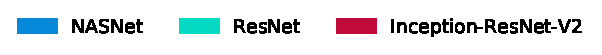
\includegraphics[scale=1]{graphics/matplot/img-class__legend.pdf}
  \begin{subfigure}[b]{0.5\linewidth}
    \centering
    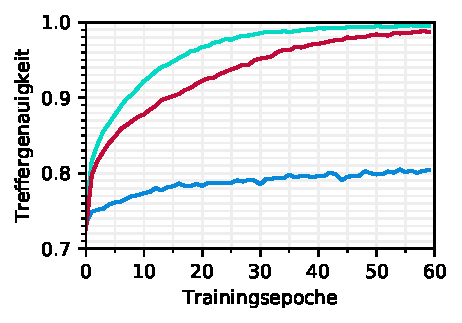
\includegraphics[scale=1]{graphics/matplot/img-class__acc.pdf}
    \caption{Trefferquote} 
    \label{image-class-results:a} 
    \vspace{2ex}
  \end{subfigure}%% 
  \begin{subfigure}[b]{0.5\linewidth}
    \centering
    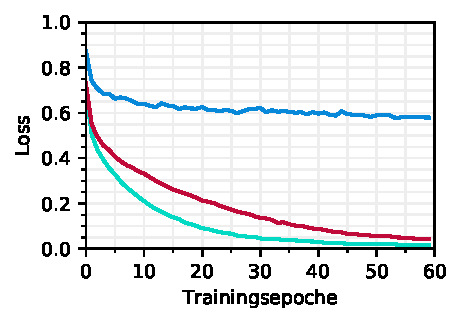
\includegraphics[scale=1]{graphics/matplot/img-class__loss.pdf}
    \caption{Loss} 
    \label{image-class-results:b} 
    \vspace{2ex}
  \end{subfigure} 
  \begin{subfigure}[b]{0.5\linewidth}
    \centering
    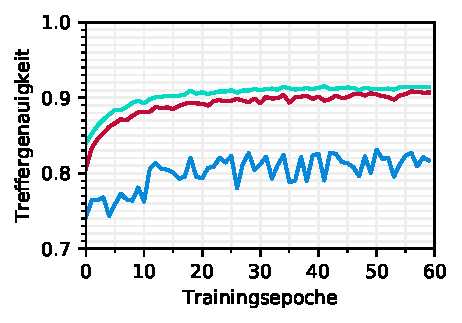
\includegraphics[scale=1]{graphics/matplot/img-class__val_acc.pdf}
    \caption{Trefferquote bei den Testdaten} 
    \label{image-class-results:c} 
  \end{subfigure}%%
  \begin{subfigure}[b]{0.5\linewidth}
    \centering
    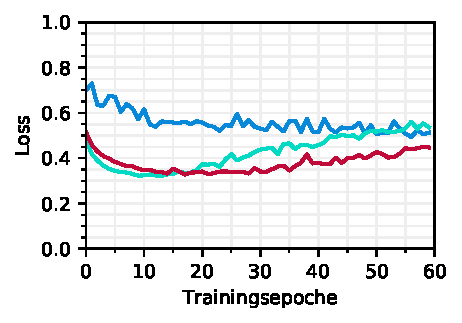
\includegraphics[scale=1]{graphics/matplot/img-class__val_loss.pdf}
    \caption{Loss bei den Testdaten} 
    \label{image-class-results:d} 
  \end{subfigure}
  \centering
\end{figure}

% Die einzelnen Modelle zeigen eine Trefferquote von TODO\% (ResNet, Epoche TODO), TODO\% (Inception-ResNet-V2, Epoche TODO) beziehungsweise TODO\% (NASNet, Epoche TODO).

% Das auf dem TODO TODO TODO\todo{TODO} basierende Modell hat mit einer Trefferquote von \todo{TODO}\% nach \todo{TODO} Epochen die höchste Trefferquote auf den Testdaten. 

Auffällig ist das schlechte Resultat des NASNet Modells. Obwohl das NASNet als eines der genausten Klassifizierungsmodelle für Bilder gilt, schneidet es im vorliegenden Experiment mit Abstand am schlechtesten ab. Wie in Abbildung \ref{image-class-results:c} ersichtlich ist, liegt die Trefferquote ungefähr bei 0.8 und somit knapp 0.2 unter den beiden anderen Modellen.

Eine fundierte Erklärung, weshalb das NASNet Modell so schlecht abschneidet, kann nicht gefunden werden. Eine mögliche Erklärung ist der mit Abstand kleinere Feature-Vektor des NASNets. Dieser ist mit nur 4'032 Neuronen wesentlich kleiner als jener des ResNet (26'6240 Neuronen) und des Inception-ResNet-V2 (13'5168 Neuronen).

Die Ergebnisse des ResNet und des Inception-ResNet-V2 sehen dagegen wesentlich besser aus. Die Modelle weisen bereits nach 30 Epochen ein Bias von weniger als 5\% (ResNet) respektive weniger als 2\% (Inception-ResNet-V2) auf. Nach 60 Epochen Training weisen die beiden Modelle ein Bias von weniger als 1.5\% respektive 0.5\% auf. Dies zeigt, dass die gewählten Modelle lernen und grundsätzlich geeignet sind, die Problemstellung anzugehen. 

Neben der auch nach 60 Epochen noch leicht steigenden Trefferquote hat das Loss auf den Testdaten (vgl. Abbildung \ref{image-class-results:d}) bereits nach 25 (ResNet) respektive 15 (Inception-ResNet-V2) Epochen den Wendepunkt erreicht. Dies zeigt, dass das Modell zu wenig gut generalisiert. Die steigende Testgenauigkeit vermittelt zwar einen guten Eindruck, das steigende Loss zeigt jedoch, dass das Modell in seinen Entscheidungen immer unsicherer wird, das heisst die Wahrscheinlichkeit, mit welcher sich das Modell sicher ist, eine Rechnung einer bestimmten Klasse zuzuweisen, sinkt. Das Modell beginnt also nach nur wenigen Epochen auswendig zu lernen (Overfitting).

Das Problem des Overfitting könnte womöglich durch zusätzliche Trainingsdaten gemindert werden, diese stehen jedoch nicht zur Verfügung.

% Im folgenden Kapitel wird ein weiterer Ansatz zur Klassifizierung der Rechnungen gezeigt, welcher mit den vorhandenen Datensätzen bessere Ergebnisse erzielen kann.

% Optimierungspotential:

% - https://towardsdatascience.com/deep-learning-performance-cheat-sheet-21374b9c4f45

% ENAS: https://github.com/carpedm20/ENAS-pytorch
% Neural Architecture Search with Reinforcement Learning: https://arxiv.org/abs/1611.01578
% Neural Optimizer Search with Reinforcement Learning: https://arxiv.org/abs/1709.07417

% \textbf{Weight penalty L1 and L2}
% Improve performance and reduce overfitting -> Keeps weights in NN small
% -> Have a look at the trained model, are there huge weights? If so, highlight this as a problem


